\ifx\boi\undefined\ifx\problemname\undefined
\providecommand\sampleinputname{}
\providecommand\sampleoutputname{}
\documentclass[english]{templates/boi}
\problemlanguage{.en}
\fi
\newcommand{\boi}{Baltic Olympiad in Informatics}
\newcommand{\practicesession}{Practice Session}
\newcommand{\contestdates}{April 27 - May 1, 2018}
\newcommand{\dayone}{Day 1}
\newcommand{\daytwo}{Day 2}
\newcommand{\licensingtext}{This problem is licensed under CC BY-SA 4.0.}
\newcommand{\problem}{Problem}
\newcommand{\inputsection}{Input}
\newcommand{\outputsection}{Output}
\newcommand{\interactivity}{Interactivity}
\newcommand{\grading}{Grading}
\newcommand{\scoring}{Scoring}
\newcommand{\constraints}{Constraints}
\renewcommand{\sampleinputname}{Sample Input}
\renewcommand{\sampleoutputname}{Sample Output}
\newcommand{\sampleexplanation}[1]{Explanation of Sample #1}
\newcommand{\sampleexplanations}{Explanation of Samples}
\newcommand{\timelimit}{Time Limit}
\newcommand{\memorylimit}{Memory Limit}
\newcommand{\seconds}{s}
\newcommand{\megabytes}{MB}
\newcommand{\group}{Group}
\newcommand{\points}{Points}
\newcommand{\limitsname}{Limits}
\newcommand{\additionalconstraints}{Additional Constraints}
\newcommand{\testgroups}{
Your solution will be tested on a set of test groups, each worth a number of points.
Each test group contains a set of test cases.
To get the points for a test group you need to solve all test cases in the test group.
Your final score will be the maximum score of a single submission.
}
\fi
\def\version{jury-1}
\problemname{Пути}
{\em Граф} -- это структура, состоящая из множества {\em вершин}, и множества {\em ребер}. Каждое ребро соединяет две вершины. На иллюстрации ниже показан пример графа с $4$ вершинами и $3$ ребрами.
%For example, a road map could be a graph, if the vertices are towns or other places and the edges are roads that directly connect two places.


{\em Путь} в графе -- это последовательность из $2$ или более вершин, соединённых последовательно рёбрами. Обратите внимание, что порядок вершин играет роль. Например, ``\texttt{5-6-7}'', ``\texttt{5-7-6}'' и ``\texttt{7-6-5}'' -- это разные пути.

В данной задаче каждая вершина графа раскрашена в один из $K$ цветов. Задача состоит в том, чтобы найти количество возможных {\em путей}, в которых никакие две вершины не имеют один и тот же цвет. 

\section*{\inputsection}
На первой строке даны три целых числа: $N$ (число вершин), $M$ (число рёбер), и $K$ (число различных цветов).

%($1 \le N, M \le 3 \cdot 10^5, 1 \le K \le 5$).

На второй строке даны $N$ целых чисел между $1$ и $K$ -- цвета каждой вершины (начиная с $1$ до $N$). 

Каждая из следующих $M$ строк описывает одно ребро, и содержит два целых числа $a, b$ ($1 \le a, b \le N, a \neq b$) -- две вершины, соединённых соответствующим ребром. Две вершины не могут быть соединены более чем одним ребром.

\section*{\outputsection}
Выведите одно целое число -- количество различных путей, все вершины которых имеют разные цвета. Известно, что ответ не превышает $10^{18}$.

\section*{\constraints}
\testgroups

\noindent
\begin{tabular}{| l | l | l |}
\hline
\group & \points & \limitsname \\ \hline
1      & 23      & $1 \le N, M \le 100, 1 \le K \le 4$ \\ \hline
2      & 20      & $1 \le N, M \le 300\,000, 1 \le K \le 3$ \\ \hline
3      & 27      & $1 \le N, M \le 300\,000, 1 \le K \le 4$ \\ \hline
4      & 30      & $1 \le N, M \le 100\,000, 1 \le K \le 5$ \\ \hline
\end{tabular}

\section*{\sampleexplanation{1}}

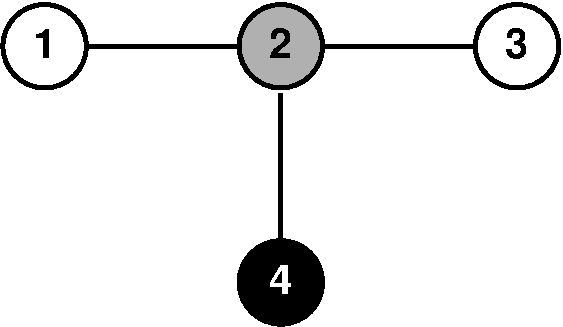
\includegraphics[width=5cm]{pathsfig.pdf}

Граф в первом примере проиллюстрирован на рисунке выше, где каждая вершина раскрашена в белый (цвет 1), серый (цвет 2) или чёрный (цвет 3). Всего есть 10 путей, в которых все вершины имеют различные цвета: ``\texttt{1-2}'', ``\texttt{2-1}'', ``\texttt{2-3}'', ``\texttt{3-2}'', ``\texttt{2-4}'', ``\texttt{4-2}'', ``\texttt{1-2-4}'', ``\texttt{4-2-1}'', ``\texttt{3-2-4}'' and ``\texttt{4-2-3}''.

Обратите внимание, что ``\texttt{1}'' не считается подходящим путём, т.к. это всего лишь одна вершина. Не подходит и путь ``\texttt{1-2-3}'', т.к. содержит две вершины цвета $1$.
